\PassOptionsToPackage{table}{xcolor}
\documentclass[9pt,xcolor=x11names,compress]{beamer}

%% General document %%%%%%%%%%%%%%%%%%%%%%%%%%%%%%%%%%
\usepackage{graphicx}
\usepackage{tikz}
\usetikzlibrary{decorations.fractals,lindenmayersystems}
\usepackage{wasysym}
%%%%%%%%%%%%%%%%%%%%%%%%%%%%%%%%%%%%%%%%%%%%%%%%%%%%%%


%% Beamer Layout %%%%%%%%%%%%%%%%%%%%%%%%%%%%%%%%%%
\useoutertheme[subsection=false,shadow]{miniframes}
\useinnertheme{default}
\usefonttheme{serif}
\usepackage{palatino}

\setbeamerfont{title like}{shape=\scshape}
\setbeamerfont{frametitle}{shape=\scshape}

\setbeamercolor*{lower separation line head}{bg=DeepSkyBlue4} 
\setbeamercolor*{normal text}{fg=black,bg=white} 
\setbeamercolor*{alerted text}{fg=DeepSkyBlue4} 
\setbeamercolor*{example text}{fg=black} 
\setbeamercolor*{structure}{fg=black} 
 
\setbeamercolor*{palette tertiary}{fg=black,bg=black!10} 
\setbeamercolor*{palette quaternary}{fg=black,bg=black!10} 

\setbeamertemplate{blocks}[rounded][shadow=true]
\setbeamercolor{block title}{bg=DeepSkyBlue4}
\setbeamercolor{block title example}{bg=DeepSkyBlue4}
\setbeamercolor{block body}{bg=black!15!white}
\setbeamercolor{block body example}{bg=black!15!white}

\setbeamertemplate{navigation symbols}{}
%%%%%%%%%%%%%%%%%%%%%%%%%%%%%%%%%%%%%%%%%%%%%%%%%%

\title{Lesson 5: The Natural Logarithm}
\author[Francisco Blanco-Silva]{Francisco Blanco-Silva}
\institute[USC]{University of South Carolina}
\date{
	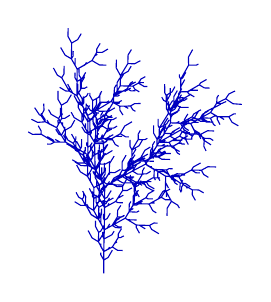
\begin{tikzpicture} 
    \draw [blue!75!black, rotate=90]
    [l-system={rule set={F -> FF-[-F+F]+[+F-F]}, axiom=F, order=4, step=2pt, 
        randomize step percent=25, angle=30, randomize angle percent=15}]
    lindenmayer system; 
	\end{tikzpicture}
	\\
}

\begin{document}

\frame{\titlepage}

\section{What do we know?}
\begin{frame}
\frametitle{What do we know?}
\begin{columns}[T]
\begin{column}{0.6\linewidth}
\begin{itemize}
\item Functions
\begin{itemize}
\item $x-$ and $y-$intercepts ($f(x)=0$, $f(0)$)
\item Change from $x=a$ to $x=b$ 
\begin{equation*}
	\Delta y = f(b)-f(a)
\end{equation*}
\item Average Rate of Change from $x=a$ to $x=b$
\begin{equation*}
ARC=\frac{\Delta y}{\Delta x}=\frac{f(b)-f(a)}{b-a} 
\end{equation*}
\item Relative Change from $x=a$ to $x=b$
\begin{equation*}
RC=\frac{\Delta y}{f(a)}=\frac{f(b)-f(a)}{f(a)}
\end{equation*}
\end{itemize}
\end{itemize}
\end{column}
\begin{column}{0.4\linewidth}
\begin{itemize}
	\item Linear Functions: $f(x)=b+mx$
	\item Exponential Functions $P=P_0\, a^t = P_0\, (1+r)^t$
\end{itemize}
\end{column}
\end{columns}
\end{frame}

\subsection{The Natural Logarithm}

\begin{frame}[t]\frametitle{Warm-up}
\framesubtitle{The Natural Logarithm}
  \begin{definition}
     The \alert{natural logarithm} of $x$, written $\ln x$, is the power of $e$ needed to get $x$:
     \begin{equation*}
      \ln x = c \text{ means } x=e^c, \text{ where } e\approx 2.7182818285
     \end{equation*}
  \end{definition}  
\end{frame}

\begin{frame}[c]\frametitle{Warm-up}
    
\framesubtitle{The Natural logarithm}

\begin{center}
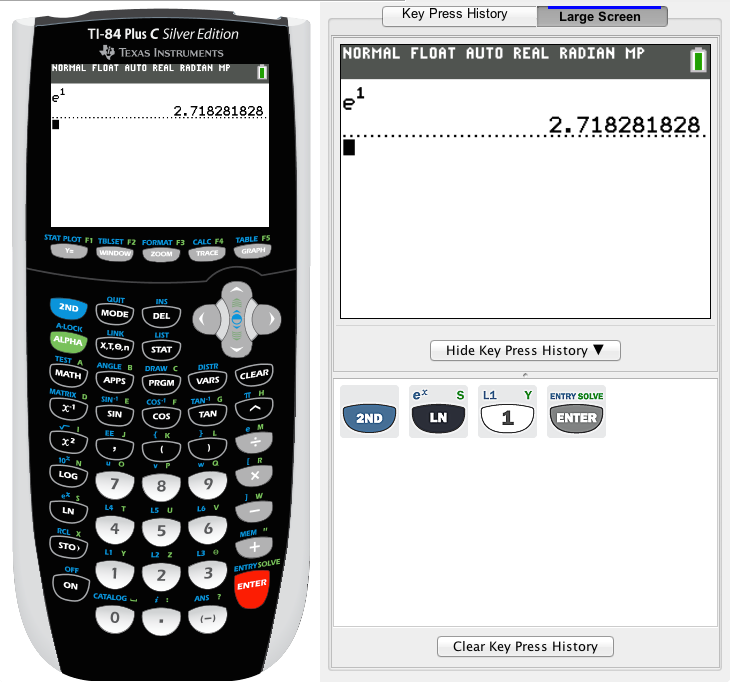
\includegraphics[height=0.8\textheight]{ti84e.png}
\end{center}
\end{frame}

\begin{frame}[t]\frametitle{Warm-up}
\framesubtitle{The Natural Logarithm}
	\begin{definition}
	   The \alert{natural logarithm} of $x$, written $\ln x$, is the power of $e$ needed to get $x$:
	   \begin{equation*}
	   	\ln x = c \text{ means } x=e^c, \text{ where } e\approx 2.7182818285
	   \end{equation*}
	\end{definition}	
	\begin{block}{Properties}
	\begin{enumerate}[<+-|alert@+>]
		\item $\ln (ab) = \ln a + \ln b$.
		\item $\ln (a/b) = \ln a - \ln b$.
		\item $\ln (a^r) = r \ln a$.
		\item $\ln e^r = r$, and $e^{\ln r} = r$.
		\item $\ln 1 = 0$, and $\ln e = 1$.
		\item $\ln x$ is not defined for $x\leq0$.
	\end{enumerate}
	\end{block}
\end{frame}

\begin{frame}[c]\frametitle{Warm-up}
    
\framesubtitle{The Natural Logarithm}

\begin{example}
Simplify the following expressions:
\begin{itemize}
  \item $\alert<2>{\ln e^6} \uncover<2->{= 6}$
  \item $\alert<3-5>{\ln 4x + 2 \ln x}$
  \begin{align*}
  \uncover<3->{\ln 4x + 2 \ln x} & \uncover<4->{= \ln 4x + \ln x^2 } \uncover<5->{= \ln 4x^3}
  \end{align*}
  \item $\alert<6-7>{- \ln x^{-1/3}} \uncover<6->{=\frac{1}{3}\ln x} \uncover<7->{\text{, or also:} - \ln x^{-1/3} = \ln x^{1/3}}$ 

  \item \alert<8->{$\ln 3x - 3 \ln x^{-1/3} - \ln 27$}
  \begin{align*}
  \uncover<8->{\ln 3x - 3 &\ln x^{-1/3} - \ln 27} \uncover<9->{= \ln 3x + \ln x - \ln 27 \\}
  \uncover<10->{&= \ln 3x^2 - \ln 27 \\}
  \uncover<11->{&= \ln \frac{3x^2}{27}} \uncover<12->{= \ln \frac{x^2}{9}}
  \end{align*}
\end{itemize}

\end{example}

\end{frame}

\begin{frame}\frametitle{Warm-up}
\framesubtitle{The Natural Logarithm}
   \begin{example}
	   Solve for $t$: 
	   \begin{equation*}
	   3^t=10
	   \end{equation*}
   \end{example} 
   \pause
   Apply the natural logarithm to both sides of the equation:
   \pause
   \begin{align*}
   	\uncover<3->{\ln 3^t &= \ln 10  \\}
   	\uncover<4->{t \cdot \ln 3 &= \ln 10 \\}
   	\uncover<5->{t &= \frac{\ln 10}{\ln 3} \approx 2.0959032737}
   \end{align*}
\end{frame}

\begin{frame}[c]\frametitle{Warm-up}
    
\framesubtitle{The Natural Logarithm}

\begin{center}
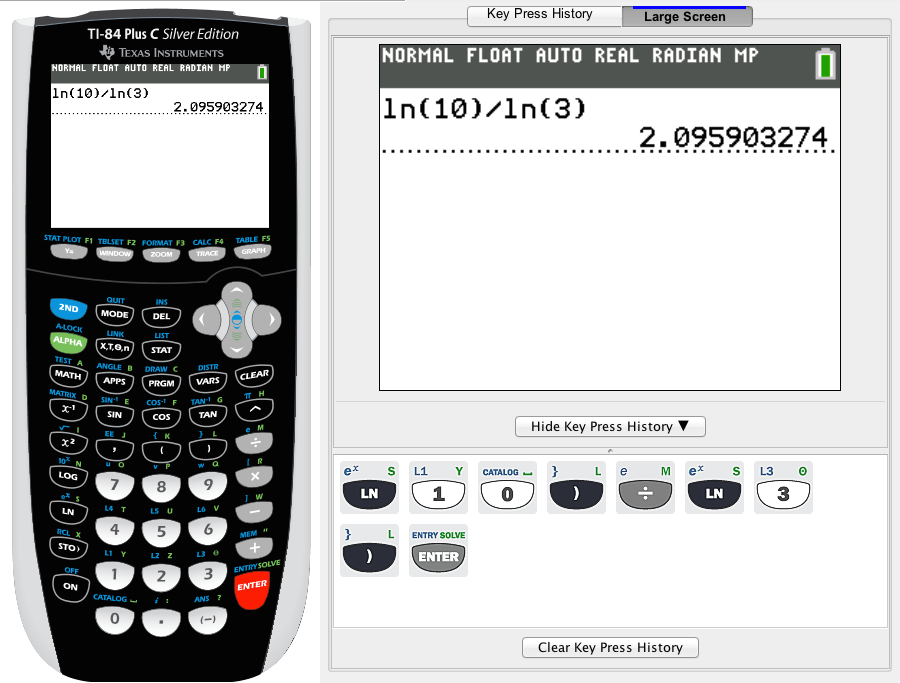
\includegraphics[width=0.9\linewidth]{ti84ln.png}
\end{center}

\end{frame}

\begin{frame}\frametitle{Warm-up}
\framesubtitle{The Natural Logarithm}
   \begin{example}
   	Solve for $t$: 
   	\begin{equation*}
   		12 = 5e^{3t}
	\end{equation*}
   \end{example}
   \pause
   \alert<2>{Before applying the natural logarithm, we force one side of the equation to be of the form $a^r$, without extra coefficients:
   \begin{equation*}
   	\only<2>{12/5}\only<3->{2.4} = e^{3t}
   \end{equation*}}
   \pause
   \alert<3>{Now we proceed as in the previous example:}
   \pause
   \begin{align*}
   	\uncover<4->{\ln e^{3t} &= \ln 2.4\\}
   	\uncover<5->{3t &=  \ln 2.4 \\}
   	\uncover<6->{t &= \frac{\ln 2.4}{3} \approx 0.2918229125}
   \end{align*}
\end{frame}

\begin{frame}\frametitle{Warm-up}
   \framesubtitle{The Natural Logarithm} 
   \begin{example}
      Write the number $a=1234$ in the form $e^k$ 
    \end{example} 
    \begin{align*}
    \uncover<2->{e^k &=1234}  \\
    \uncover<3->{\ln e^k &= \ln 1234} \\
    \uncover<4->{\alert{k} &\alert{=7.118016204 }}
    \end{align*}
    \uncover<5->{ Therefore,}
    \begin{equation*}
      \uncover<5->{1234 = e^{7.118016204}} 
    \end{equation*}
\end{frame}

\section{Exponential Functions}

\subsection{Motivation and Definition}
\begin{frame}[t] \frametitle{Exponential Functions}
\framesubtitle{Examples}
   \begin{example}
   The population of Nevada in 2000 was 2.02 million, and in 2006, 2.498 million.  Assuming that the growth obbeys an exponential law, find a formula as a function of $t$ years after 2000. \alert{When will the population reach 4 million?}
   \end{example} 
   \uncover<2->{\alert<2>{We need a function of the form $P=P(t)=P_0 a^t$ (in millions), with $t$ in years after 2000.  It must be $P_0=2.02$.}} \uncover<3->{\alert<3>{To find the value of $a$, we use:
   \begin{align*}
    P(6)&=2.02 a^6 =2.498 &a &=\Big( \frac{2.498}{2.02} \Big)^{1/6} \approx 1.036
   \end{align*}}}
   \uncover<4->{\alert<4>{It is then $P = 2.02 (1.036)^t$.}}

   \uncover<5->{\alert<4>{In order to answer the second question, we must then solve for $t$ in the following equation:
   \begin{equation*}
    2.02(1.036)^t = 4 
   \end{equation*}}}
\end{frame}


\begin{frame}[t]\frametitle{The Natural Logarithm}
\framesubtitle{Examples}
\begin{example}
   The population of Nevada in 2000 was 2.02 million, and in 2006, 2.498 million.  Assuming that the growth obbeys an exponential law, find a formula as a function of $t$ years after 2000. \alert{When will the population reach 4 million?}
   \end{example} 
\begin{align*}
\uncover<2->{2.02 (1.036)^t &= 4} \uncover<5->{&\ln (1.036^t) &= \ln 1.9801980198} \\
\uncover<3->{1.036^t &= \frac{4}{2.02}} 
\uncover<6->{&\ln (1.036)\cdot t &= 0.6831968497}\\
\uncover<4->{1.036^t &= 1.9801980198} \uncover<7->{&t &= \frac{0.6831968497}{0.035367143845} }\\
&\uncover<8->{&\alert<9>{t} &\alert<9>{\approx 19.317275175}}
\end{align*}
\only<9>{\alert{Solution: In 2019.}}
\end{frame}

\subsection{Motivation}
\begin{frame}\frametitle{Exponential Functions}
   \framesubtitle{Applications of the Natural Logarithm} 
   We are able to \emph{rewrite} the expression of any exponential function $P=P_0a^t$ using the number $e$ as the base, instead.  The function will look different, but will keep its value!

   \pause All we need to do is re-write $a$ as a power of $e$ ($e^k=a$) and use logarithms to find the value of $k$:
   \begin{align*}
   	\uncover<3->{e^k&=a \\}
   	\uncover<4->{\ln e^k &=\ln a \\}
   	\uncover<5->{k &= \ln a}
   \end{align*}

   \uncover<6->{And so, \alert{$P=P_0\, a^t = P_0\, (e^k)^t = P_0\, e^{kt}$}}
\end{frame}

\subsection{Summary}
\begin{frame}\frametitle{Exponential Functions}
   \framesubtitle{Applications of the Natural Logarithm} 
\begin{block}{In Summary}
	Every exponential function can be written in three different ways:
	\begin{equation*}
		P = P(t) = P_0\, a^t = P_0\, (1+r)^t = P_0\, e^{kt}	
	\end{equation*}
\end{block}
\begin{itemize}
	\item $P_0$ is the initial value
	\item $a$ is the base
	\item $r$ is the \alert{growth/decay rate}
	\item We refer to $k$ as the \alert{continuous growth/decay rate}
\end{itemize}
	The values of $a$, $r$ and $k$ are related, of course:
	\begin{align*}
		a&=1+r &k&=\ln a	&k&=\ln(1+r) \\
    \uncover<2->{r&=a-1 &a&=e^k &r&=e^k-1}
	\end{align*}
\end{frame}

\subsection{Warm-up}
\begin{frame}\frametitle{Exponential Functions}
  \framesubtitle{Applications of the Natural Logarithm}  
  \begin{example}
  \begin{itemize}
    \item \alert<2-4>{Write the function $P=15(1.5)^t$ in the form $P=P_0e^{kt}$}
    \item \alert<5->{Write the function $P=174e^{0.3t}$ in the form $P=P_0 a^t$}
  \end{itemize}
  \end{example}
  \begin{itemize}
    \item<2-> They are giving us $a$ and asking for $k$.  We need to use the relation $k=\ln a$.
    \begin{equation*}
      \uncover<3->{k = \ln 1.5 = 0.4054651081}
    \end{equation*}
    \pause\pause\pause
    Therefore, the solution of this part is 
    \begin{equation*}
      P=15e^{0.4054651081\, t}
    \end{equation*}
    \item<5-> They are giving us $k$ and asking for $a$.  We neet to use the relation $a=e^k$.
    \begin{equation*}
      \uncover<6->{a=e^k=e^{0.3}=1.349858808}
    \end{equation*}
    \pause\pause\pause Therefore, the solution of this part is
    \begin{equation*}
      \alert{P=174(1.349858808)^t}  
    \end{equation*}
  \end{itemize}
\end{frame}

\begin{frame} \frametitle{Exponential Functions}
   \framesubtitle{Applications of the Natural Logarithm} 
   \begin{example}
    Let $P=100 e^{0.04t}$ with time $t$ in years.
    \begin{itemize}
        \item \alert<2>{What is the continuous percent growth rate?}
        \item \alert<3->{What is the annual percent growth rate?}
      \end{itemize} 
   \end{example}
   \begin{itemize}
    \item<2-> This is direct from the function, since they are giving us $k=0.04$.  The continuous percent growth rate is 4\%.
    \item<3-> For the annual (not continuous!) percent growth rate, we need to find the value of $r$ first.  We need to use the relation $r=e^k-1$.
    \begin{equation*}
      \uncover<4->{r=e^k-1=e^{0.04}-1=0.040810774}
    \end{equation*}
    \pause\pause\pause\pause \alert{The annual growth rate is then 4.081\%}
   \end{itemize}
\end{frame}

\end{document}